%%%%%%%%%%%%%%%%%%%%%%%%%%%%%%%%%%%%%%%%%%%%%%%%%%%%%%%%%%%%%%%%%
\chapter{CONDITION MONITORING OF INDUCTION MOTORS: BACKGROUND }\label{Ch2}
%%%%%%%%%%%%%%%%%%%%%%%%%%%%%%%%%%%%%%%%%%%%%%%%%%%%%%%%%%%%%%%%%
\vspace*{-12pt} % If no text above section, use this vspace* to lift the whole part to the proper starting point - SBÖ
\section{Introduction of Induction Motors}
\subsection{Principle of operation}

Electric motors are divided into two classes depending on their power supply type: direct current (DC) or alternating current (AC). The latter can be broken into two classes as synchronous or induction according to their operating speed. Induction motors, which operates slightly lower than synchronous speed, are also sub-divided as wounded and squirrel-cage motors. In this study, squirrel-cage induction motors have been investigated by means of induction motors, since the squirrel-cage type is predominantly used in industrial applications. 

Induction motors run at a speed slightly lower than synchronous speed at the point where motor torque and load torque are equal \cite{gunnar2016}. The difference between the actual rotor speed and synchronous speed is called as slip \cite{doe2008improving}.

\begin{equation}
	\text{Synchronous Speed} = \displaystyle \frac{120 \cdot \text{Frequency (Hz)}}{\text{number of poles}}
	\label{speed}
\end{equation}

\begin{equation}
	\text{Slip} = \displaystyle \frac{\text{Synchronous Speed - Rotor's Mechanical Speed}}{\text{Synchronous Speed}}
	\label{slip}
\end{equation}

%\begin{figure}[h]
%	\centering
%	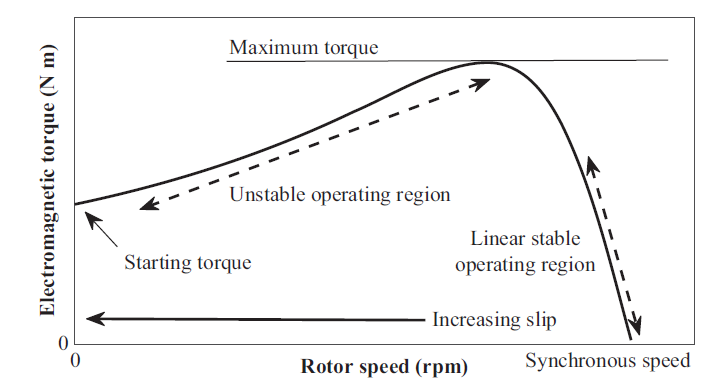
\includegraphics[width=250pt,keepaspectratio=true]{./fig/torque_speed.PNG}
%	% sekil3.eps: 0x0 pixel, 300dpi, 0.00x0.00 cm, bb=14 14 1155 740
%	\caption{Steady-state torque-speed curve of an induction motor, adapted from \cite{faiz2017fault}.}	
%	\label{ts}
%\end{figure}

In Principle, induction motors transfer electrical energy into mechanical energy by interlinking two electrical components: stator as stationary part and rotor as rotational part. Electrical energy transmitted from stator to rotor via electromagnetic induction, then a mechanical component bearing guides rotor to provide mechanical power \cite{oliver1992electric,karmakar2016induction}.

\begin{figure}[h]
	\centering
	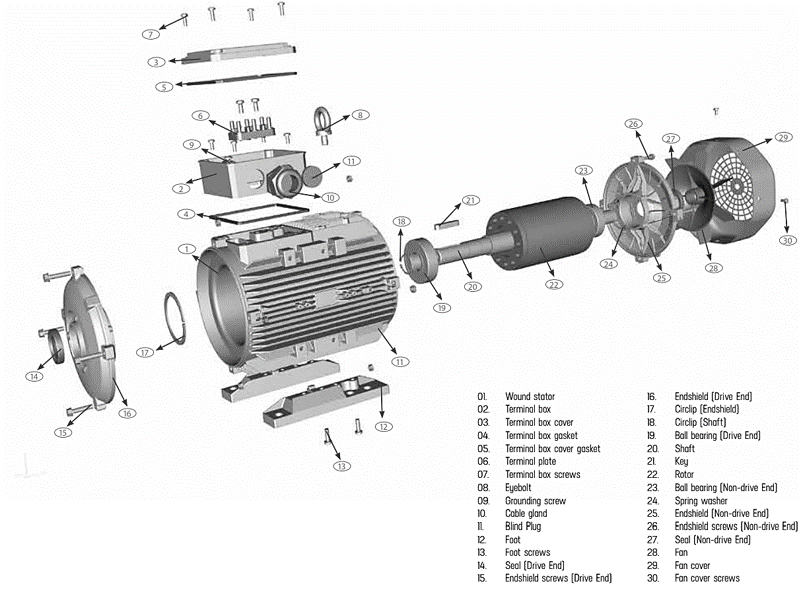
\includegraphics[width=350pt,keepaspectratio=true]{./fig/watmotor.PNG}
	% sekil3.eps: 0x0 pixel, 300dpi, 0.00x0.00 cm, bb=14 14 1155 740
	\caption{Squirrel cage induction motor structure, courtesy of WAT Motor Co.}	
	\label{motor}
\end{figure}

\subsection{VFD-fed induction motors}

A variable frequency drive, also called as inverter, adjustable-frequency drive (AFD) or variable-speed drive (VSD), fed motor system controls the rotation speed of the induction motor by controlling the supply frequency and voltage of the motor. The main difference between line-start and VFD-fed induction motors is that while in line-start mode supply voltage is the only controllable parameter, on the other hand, VFD-fed has the ability to control torque and speed easily \cite{faiz2017fault}.

% \begin{figure}[h]
% 	\centering
% 	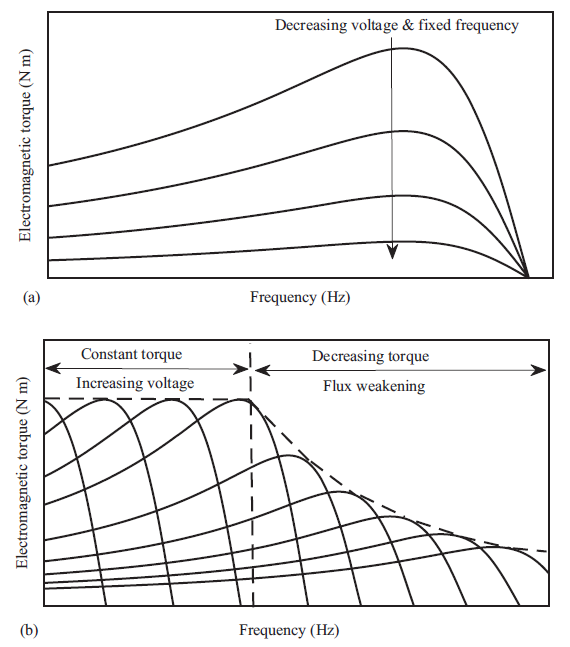
\includegraphics[width=250pt,keepaspectratio=true]{./fig/vfd.PNG}
% 	% sekil3.eps: 0x0 pixel, 300dpi, 0.00x0.00 cm, bb=14 14 1155 740
% 	\caption{(a) Torque–speed curves for different voltages in line-start operation and (b) Torque–speed curves for different voltages and frequencies in VFD-fed operation, adapted from \cite{faiz2017fault}.}	
% 	\label{vfd}
% \end{figure}

From a historical point of view, DC motors have been utilised in speed control applications. However, as a result of advances in power semiconductor technology used in inverters, the performance of AC motors in terms of precision, response, and speed range began to exceed that of DC motors \cite{doe2008improving,mikami2011historical}. As a driving force behind the induction motor control dominance today, VFDs generally have the following control strategies regarding speed and torque regulation \cite{weg,danfoss}:

\begin{itemize}
	\item Voltage per Frequency Control (V/f)
	\item Field Oriented Control (FOC)
	\item Direct Torque Control (DTC)
\end{itemize}

The common idea behind these methods is based on controlling the torque and flux references applied to the motor separately, as in DC motor control \cite{faiz2017fault}. In the scope of this thesis, only the V/f control strategy emphasized due to the widespread adoption of the control method in pump, compressor and fan applications. 

V/f control can be employed in both open-loop and closed-loop modes. Open-loop V/f control, which is by far the most popular control due to its simplicity, as the name implies, creates a constant air-gap flux by keeping the ratio between the voltage and frequency applied to the induction motor constant, and as a result, it provides the opportunity to work at operating frequencies from zero to nominal frequency \cite{bose2002modern}. 

VFDs come with benefits such that energy savings, reliability and product quality, yet in concern of fault diagnosis they introduce a number of factors, which will be discussed later on, that increase the complexity. 

\subsection{Need for condition monitoring}

Condition monitoring defined as measuring activities concerning characteristics and parameters of physical equipment at predetermined intervals either manually or automatically \cite{en201713306}. Leveraging rapid technological advancements in data storage, data process and network structure, condition monitoring became one of the driving force behind the industry 4.0 paradigm. The key goal behind this paradigm is to acquisition, transmission and analysis of data in order to predict future behaviours of machinery, or plant on a larger scale, to boost efficiency and reliability \cite{lughofer2019prologue,RUIZSARMIENTO}. 

Researchers from both academia and industry have devoted significant attention to condition monitoring of induction motors over decades. Even though induction motors renowned for robustness, environmental, electrical and mechanical effects may lead induction motors to failure. As a result, industrial processes subjected to potential losses in a manner of time and capital, so the desire to minimize or even prevent these losses emerges the need for condition monitoring. 

\subsection{Maintenance strategies}

Maintenance can be defined as the combination of all technical and managerial actions taken to maintain or restore an item throughout its life cycle in a condition where it can fulfil its designed function \cite{en201713306}. A motor maintenance program should effectively address reliability, cost, and scheduling issues, as well as the causes of the most common motor failures. Essentially, there are two types of maintenance strategies: corrective and preventive. 

\begin{figure}[h]
	\centering
	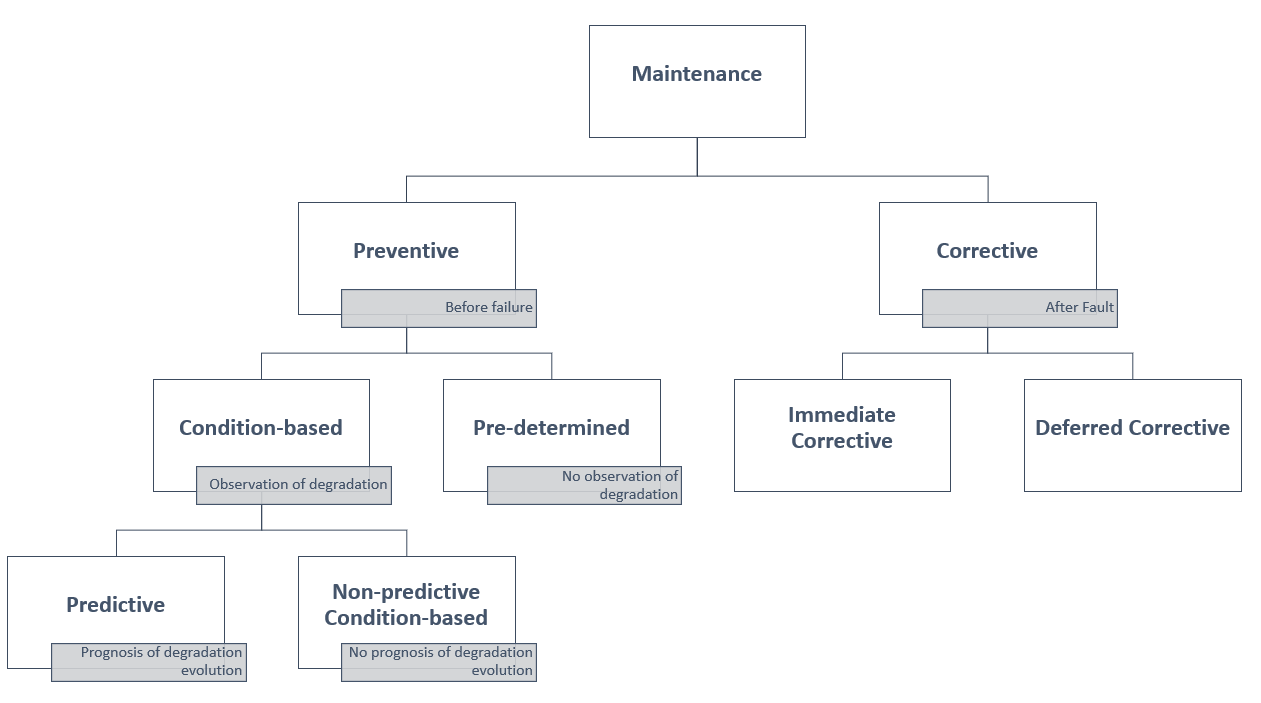
\includegraphics[width=400pt,keepaspectratio=true]{./fig/maintenance.PNG}
	% sekil3.eps: 0x0 pixel, 300dpi, 0.00x0.00 cm, bb=14 14 1155 740
	\caption{Maintenance types, adapted from \cite{en201713306}.}	
	\label{maintenance}
\end{figure}

Corrective maintenance is a type of maintenance performed after the induction motor failure to detect the fault and restore it to operational condition \cite{en201713306}. The main purpose of this type of maintenance is to get the equipment up and running as soon as possible by repairing or replacing the defective equipment. However, corrective maintenance as a failure-driven method contains a high-risk potential as faults may occur at unexpected times, can disrupt the operation. Since this type of maintenance approach does not take into account the damages that may occur, it may be suitable for equipment that is not critical to the business that does not pose a safety risk.

Preventive maintenance, on the other hand, aims to detect faults at an early step and correct them before they create risk to operation \cite{en201713306}. Preventive maintenance employed to increase efficiency and reliability by taking into account the probability of failure or the ageing of the equipment, at certain intervals or according to pre-planned scheduling. Although this approach is beneficial in cases where the wear-out characteristics are evident, it has disadvantages, especially in terms of not being able to use equipment lifespan efficiently and increasing the maintenance cost compared to the corrective maintenance approach \cite{AHMAD}.

Predictive maintenance is a condition-based approach to maintenance that is used to evaluate the parameters and characteristics of the equipment or to make predictions based on repeated analysis \cite{en201713306}. Compared to preventive maintenance, predictive maintenance maximizes equipment service-life whilst minimizing unnecessary maintenance. In 99\% of machine failures, it is possible to observe indications that malfunctions will occur, in other words, the necessary measures can be taken before 99\% of the faults occur by continuously monitoring the machine \cite{AHMAD}.

Within the predictive maintenance approach, decision-making can be divided into two: diagnosis, which is the analysis of the current situation, and prognosis, which is the assessment of conditions measured over time \cite{tinga2019physical}. A P-F curve can be used to better understand diagnostic and prognostic monitoring systems.

\begin{figure}[h]
	\centering
	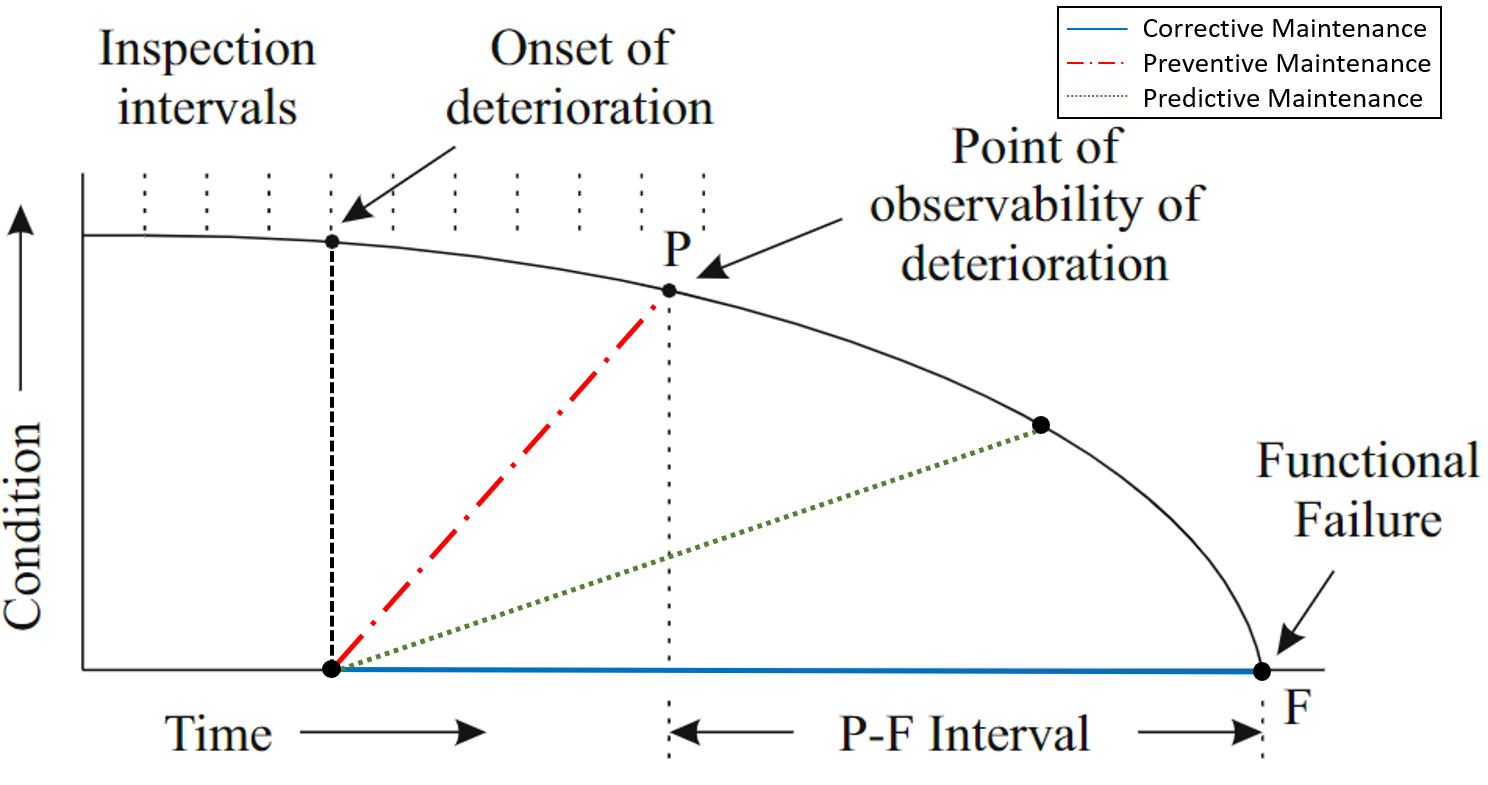
\includegraphics[width=300pt,keepaspectratio=true]{./fig/PFdiagram.png}
	% sekil3.eps: 0x0 pixel, 300dpi, 0.00x0.00 cm, bb=14 14 1155 740
	\caption{The P-F curve shows the point where the fault started, became observable and the fault occurred, adapted from \cite{tinga2019physical}.}	
	\label{PF_diagram}
\end{figure}

The downside of predictive maintenance is that it requires additional equipment and relatively high investment costs. But the advantage of VFDs also comes out here. As they currently monitor motor parameters in control applications, they have a high potential for predictive maintenance applications without the need for additional sensors and investments.

% \vspace{6pt}
% \begin{figure}[h]
% 	\centering
% 	
\includegraphics[scale=.3]{./fig/sekil1}
% 	% sekil1.eps: 0x0 pixel, 300dpi, 0.00x0.00 cm, bb=14 14 592 479
% 	\vspace{6pt}
% 	\caption{All tables and figures must be horizontally centered on the page.}
% 	\label{Figure2.1}
% \end{figure}

% %\begin{figure}
% %	\begin{minipage}[b]{.5\linewidth}
% %		\centering
% %		
\includegraphics[scale=.2]{./fig/sekil1}
% %		\subcaption{A subfigure}\label{Figure2.2a}
% %	\end{minipage}
% %	\begin{minipage}[b]{.5\linewidth}
% %		\centering
% %		
\includegraphics[scale=.2]{./fig/sekil1}
% %		\subcaption{Another subfigure}\label{Figure2.2b}
% %	\end{minipage}
% %	\caption{A figure}\label{Figure2.2} % If no need a caption for main figure comment it out 
% %\end{figure}
% %%Figure letter: \subref{Figure2.2a}

% %\begin{figure}
% %	\begin{subfigure}[b]{.5\linewidth}
% %		\centering
% %		
\includegraphics[scale=.2]{./fig/sekil1}
% %		\caption{A subfigure}\label{Figure2.3a}
% %	\end{subfigure}
% %	\begin{subfigure}[b]{.5\linewidth}
% %		\centering
% %		
\includegraphics[scale=.2]{./fig/sekil1}
% %		\caption{Another subfigure}\label{Figure2.3b}
% %	\end{subfigure}
% %	\caption{A figure}\label{Figure2.3}
% %\end{figure}

% % Subfigure example with proper LOF usage - SBÖ
% \begin{figure}[h]
% 	\centering
% 	\begin{subfigure}{.8\textwidth}
% 		\centering
% 		
\includegraphics[scale=.3]{./fig/sekil1}
% 		\firstsubcaption{First subcaption of the subfigure.}
% 		\label{Figure2.2a}
% 	\end{subfigure}
% 	\begin{subfigure}{.8\textwidth}
% 		\centering
% 		
\includegraphics[scale=.3]{./fig/sekil1}
% 		\nextsubcaption{Second subcaption of the subfigure.}
% 		\label{Figure2.2b}
% 	\end{subfigure}
%     \caption{An example of subfigure main caption.}\label{Figure2.2}
% \end{figure}

% %\begin{figure}
% %	\centering     % not \center
% %	\subcaption[]{Another subfigure}{\label{fig:a}
\includegraphics[scale=.2]{./fig/sekil1}}
% %	\subcaption[]{Another subfigure}{\label{fig:b}
\includegraphics[scale=.2]{./fig/sekil1}}
% %	%\caption{(a) this is fig 1 (b) this is fig 2.}
% %	\label{L50}
% %\end{figure}

% In Figure \ref{Figure2.2}, sed diam nonumy eirmod tempor invidunt ut labore et dolore magna aliquyam erat, sed diam voluptua. At vero eos et accusam et justo duo dolores et ea rebum. Lorem ipsum dolor sit amet, consetetur sadipscing elitr, sed diam nonumy eirmod tempor invidunt ut labore et dolore magna aliquyam erat, sed diam voluptua. At vero eos et accusam et justo duo dolores et ea rebum. At vero eos et accusam et justo duo dolores et ea rebum. At vero eos et accusam et justo duo dolores et ea rebum. At vero eos et accusam et justo duo dolores et ea rebum. At vero eos et accusam et justo duo dolores et ea rebum. At vero eos et accusam et justo duo dolores et ea rebum. At vero eos et accusam et justo duo dolores et ea rebum in Figure \ref{Figure2.2a}.

% \begin{figure}
% 	\centering
% 	
\includegraphics[width=10cm,keepaspectratio=true]{./fig/sekil2}
% 	% sekil2.eps: 0x0 pixel, 300dpi, 0.00x0.00 cm, bb=14 14 818 556
% 	\vspace{3pt}
% 	\caption{Example figure.}
% 	\label{Figure2.3}
% \end{figure}
% \vspace{-6pt}
\section{Induction Motor Fault Types}

From a mechanical perspective, induction machines basically consist of three components: stator, rotor and bearing. Electrical, mechanical, and environmental disturbances constantly affect asynchronous motor components and cause most malfunctions \cite{bonnet2010}. Table \ref{Table2.1} exhibits various surveys that studied and categorized the most common failures \cite{motor1985report,albrecht1986assessment,albrecht1987assessment,thorsen1995survey,bonnett2008increased}. 

\begin{table*}[h]
	{\setlength{\tabcolsep}{12pt}
		\caption{Distribution of induction motor faults by component (\%).}
		\begin{center}
			\vspace{-6mm}
			\begin{tabular}{ccccc}
				\hline \\[-2.45ex] \hline \\[-2.1ex]
				Component & IEEE & EPRI & Thorsen-Dalva & Bonnett-Yung \\
				\hline \\[-1.8ex]
				Bering & 44 & 41 & 51 & 69 \\
				Stator & 26 & 37  & 16 & 21\\
				Rotor & 8 & 10 & 5 & 7 \\
				Other & 22 & 12  & 28 & 3\\
				\hline
			\end{tabular}
			\vspace{-6mm}
		\end{center}
		\label{Table2.1}}
\end{table*}

Considering the actual distribution of the faults, in total 80\% of the faulty motors have only one fault, while this rate reaches 90\% especially in low voltage supply motors \cite{albrecht1987assessment}.

\begin{table*}[h]
	{\setlength{\tabcolsep}{12pt}
		\caption{Actual distribution of multiple failures (\%)) \cite{albrecht1987assessment}.}
		\begin{center}
			\vspace{-6mm}
			\begin{tabular}{ccccc}
				\hline \\[-2.45ex] \hline \\[-2.1ex]
				\multirow{2}{*}{Exact Failure} & \multicolumn{3}{c}{Motor Supply Voltage} & \multirow{2}{*}{Total} \\
				& Low  & Middle & High &      \\
				\hline \\[-1.8ex]
				1 Fault   & 91.1 & 79.6   & 77.1 & 79.9 \\
				2 Faults  & 8.0  & 11.8   & 13.1 & 11.9 \\
				3 Faults  & 0.9  & 3.3    & 5.5  & 4.0  \\
				4 Faults  & 0.0  & 2.2    & 0.8  & 1.3  \\
				> 4 Faults & 0.0  & 3.0    & 3.5  & 2.9  \\
				\hline
			\end{tabular}
			\vspace{-6mm}
		\end{center}
		\label{Table2.2}}
\end{table*}

As can be seen in Table \ref{Table2.1}, most of the faults associated with bearings followed by stator related faults. It also should be noted that these surveys do not include the effects of power electronics. A motor controlled by VFD is subjected to short and high voltage pulses called PWM (Pulse Width Modulation), which are sent at a very high frequency, which can have a detrimental effect on the wire insulation and cause a burn on the stator \cite{gunnar2016}. Although this problem can be solved with high-quality insulation, PWM signals also create non-continuous electrical discharges on the bearings, causing wear which reduces bearing lifespan \cite{trigeassou2013electrical}. Therefore, it would not be wrong to conclude that bearing and stator failures will also have a high rate in VFD-fed induction motors.

\subsection{Bearing related faults}

In all kinds of electrical machines, the mechanical element positioned between the frame that initiates the movement and the rotating axis shaft is called a bearing. These mechanical elements, which help the rotational movement of the electric motor, are exposed to many internal and external destructive effects during their operation and failures arise as a result. Major sources of bearing failures are given below \cite{zhang2010survey,easa,skf,schoen1995motor,en201320958,bonnet2010}:

\textbf{Mechanical stresses}: Fatigue, which mostly begins on the surface, turns into small-sized material ruptures at the beginning and later dimensional surface indentations and protrusions. Loose motor connection, misalignment where the motor shaft and load shaft are connected without aligning on the same axis, angular misalignment where the motor shaft and load shaft axes are connected at a certain angle, and unbalanced load connection, which is an unbalance condition where the centre of gravity of the load connected to the motor shaft is not on the rotation axis are other mechanical disturbances on the bearing.

\textbf{Environmental stresses}: Corrosion occurs on the bearing surfaces used in high humidity working environments. Especially the moisture absorbed in the bearing oil initiates this process and the rust that occurs due to corrosion causes deterioration that turns into indentation and protrusion on the surface of the bearing element, and cracks in the later stages.

\textbf{Thermal stresses}: Insufficient lubrication generally causes problems with bearing components. Normally, there is a layer of oil in the bearing that prevents direct contact between the rotating elements so that their surfaces do not wear out quickly. In case of insufficient lubrication, excessive wear and subsequent material deterioration occur as a result of increased friction due to direct contact between metal surfaces.

\textbf{Electrical stresses}: the electrical discharge current effect occurs with a fault current flowing through the bearings from the motor frame to the ground in motors that do not have a suitable ground connection. Asymmetry of stator windings, permanent magnetism effect developing in the motor over time, electrostatic charge accumulation in the motor frame and application of voltage to the motor shaft from the outside, or common end voltages generated due to the high switching frequency of semiconductor power electronics (VFDs using PWM) are the factors that cause this malfunction. The irregular current will cause wear and tear on the bearing metal surface, and as a result, the degree of material rupture and surface deterioration increases.

Vibration in the motor causes the rotor to rotate irregularly or axially unbalanced in the motor air gap. Any axial misalignment that occurs in the motor air gap adversely affects the air gap flux density and causes the formation of harmonic components \cite{schoen1995motor,en201320958,faiz2017fault}. Consequently, this can induce harmonic components in the current drawn by the motor with frequencies given by formula \cite{schoen1995motor}:
\begin{equation}
	f_{bng}=f_{e} \pm m \cdot f_{\mathrm{v}}
	\label{bearingfault}
\end{equation}
where,\\
$f_{e} \quad$ is the electrical supply frequency;\\
$f_{\mathrm{v}} \quad$ is the rotational speed frequency of the rotor;\\
$\mathrm{m} \quad$ is the harmonic number $1,2,3 \ldots$..;\\
$f_{bng} \quad$ is the current component frequency due to air gap changes.

\subsection{Stator related faults}

As researches have shown, stator faults occupy an important place among asynchronous motor faults after bearing \cite{motor1985report,albrecht1986assessment,albrecht1987assessment,thorsen1995survey,bonnett2008increased}. Mechanical, electrical, thermal and environmental factors cause malfunctions in the stator windings, as well as their laminations \cite{karmakar2016induction,Siddique}. Winding faults, as the most common stator faults, are winding short-circuit faults that are mostly the result of the aforementioned effects of the winding insulation. Types of winding faults are as follows \cite{karmakar2016induction,Siddique,lipo}:

\begin{itemize}
	\item Short-circuit between two turns in the same phase (turn-turn failure),
	\item Short-circuit between two coils side by side in the same phase (coil-coil failure),
	\item Short-circuit between the turns of two phases (phase-phase failure),
	\item Short-circuit consisting of all three-phase turns,
	\item Short-circuit between the conductor of the winding and the stator core (phase-ground short circuit),
	\item Open-circuit fault when winding breaks.
\end{itemize}

\begin{figure}[h]
	\centering
	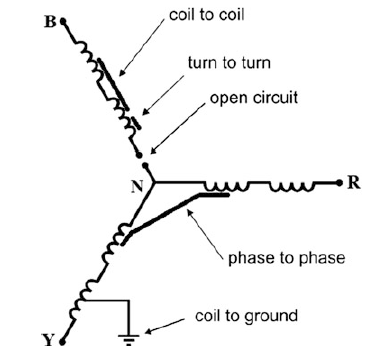
\includegraphics[width=150pt,keepaspectratio=true]{./fig/stator.PNG}
	% sekil3.eps: 0x0 pixel, 300dpi, 0.00x0.00 cm, bb=14 14 1155 740
	\caption{Star-connected stator winding faults, adapted from \cite{karmakar2016induction}.}	
	\label{statorwinding}
\end{figure}

The factors that cause the motor winding insulation to deteriorate are explained below \cite{bonnett1999root,karmakar2016induction,Siddique,faiz2017fault}:

\textbf{Mechanical stresses}: While the motor is running, the rotor may rub or hit the inner surface of the stator due to motor shaft deterioration, bearing failures and misalignment. This force creates a turn-to-turn or a phase-to-earth short-circuit, causing the stator coil and the stator winding insulation to break down. On the other hand, winding breakage may occur due to vibration during operation and therefore the motor produces the open-circuit fault.

\textbf{Environmental stresses}: The environment in which the motor is running can be very hot, cold or humid. On the other hand, substances in the external environment can contaminate the windings, causing the heat dissipation to deteriorate and the insulation to be damaged. In addition, the airflow can be blocked and cannot absorb the air required for cooling. Therefore, it causes the motor windings to heat and consequently the insulation to deteriorate.

\textbf{Thermal stresses}: Thermal effects occur as a result of overloading or a motor failure. With motor overload, the motor temperature rises above the limit value of the insulation class and the insulation deteriorates. At this point, every 3.5\% unbalance in the motor supply voltage increases the temperature of the motor by 10°C. In addition, every 10°C temperature increase above the limit temperature value of the insulation halves the life of the insulation.

\textbf{Electrical stresses}: The main reason for this is sudden changes in supply voltage. Transients during commissioning and decommissioning and voltage fluctuations frequently occur, especially in asynchronous motors powered by variable frequency drives. Winding insulations deteriorate due to these voltage variations.

Under the inter-turn short-circuit condition, a significant deviation in rotor slot harmonics components, called as principle slot harmonics (PSH), occurs and can be obtained by given formula \cite{Penman};
\begin{equation}
	f_{st}=f_{e} \cdot\left[n \cdot \frac{(1-s)}{p} \pm k\right]
	\label{statorfault}
\end{equation}
where,\\
$f_{e} \quad$ is the electrical supply frequency ;\\
$\mathrm{p} \quad$ is the number of pole pairs of the motor ;\\
$\mathrm{n} \quad$ = $1,2,3 \ldots (2p-1)$;\\
$\mathrm{s} \quad$ is the slip ;\\
$\mathrm{k} \quad$ is the harmonic number $1,2,3 \ldots$..;\\
$f_{st} \quad$ is the principle slot harmonic frequencies.

\subsection{Rotor related faults}

There are several reasons why rotor bar faults can occur in an induction motor. In caged motors, breaking one cage bar does not significantly change the operating behaviour of the machine. However, due to the fracture that occurs, the current distribution, air gap flux, force balance and temperature distribution in the rotor deteriorate, and heating and strains increase \cite{imeryuz2009asenkron}. If the rotor continues to run in this state, damage can also spread to the sidebars, causing multiple bars of the rotor to break. In this respect, it is very important to diagnose the condition when a rotor bar broken.

The main reasons of rotor broken bar of an induction motor can be listed as follows \cite{imeryuz2009asenkron,filippetti2013condition,bonnett1999root,Siddique};

\textbf{Mechanical stresses}: In cases that cause structural asymmetry such as rotor misalignment or bearing failure, the resultant of the normal direction forces in the air gap is not equal to zero and the force acting on the bars increases. In addition, dynamic effects such as impact forces due to sudden load change, centrifugal forces due to excessive acceleration also cause failure.

\textbf{Environmental stresses}: Dusty, wet and/or oily environment in which the electric motor operates negatively affects the engine and increases the possibility of malfunction.

\textbf{Thermal stresses}: Thermal stresses may occur during take-off and/or operation. The temperature limit values of the motor and rotor are different. In terms of the safe operation of the motor, the rotor temperature at start-up and the stator temperature during operation are decisive. Thermal stresses are generally caused by frequent starting, locking of the motor shaft, bearing failure, insufficient cooling, skin effect and current accumulation. It takes the form of partial warming in machines fed by power electronics.

\textbf{Electrical stresses}: The flux created by the current flowing through the rotor bars creates an electrodynamic force $(F \propto I^2)$ acting from the rotor surface towards the shaft in quadratic proportion to the current. The bar vibrates at $2\cdot s\cdot f_{e}$ and $4\cdot s\cdot f_{e}$  frequencies and can therefore cause breakage in the rotor bars. In addition, since the rotor current at motor start-up is very high, the rotor bar is again exposed to high stresses.

Cracked or broken bar in the rotor cage results a series of sideband frequencies in the stator current given by \cite{karmakar2016induction};
\begin{equation}
	f_{brb}=f_{e} \cdot\left[1 \pm 2\cdot k\cdot s \right]
	\label{rotorfault}
\end{equation}
where,\\
$f_{e} \quad$ is the electrical supply frequency ;\\
$\mathrm{s} \quad$ is the slip ;\\
$\mathrm{k} \quad$ is the harmonic number $1,2,3 \ldots$..;\\
$f_{brb} \quad$ is the broken rotor bar sideband frequencies.

% % Change margins on the fly to reset the page margins to one inch - SBÖ
% \newenvironment{changemargin}[4]{
% 	\begin{list}{}{
% 			\setlength{\voffset}{#1}
% 			\setlength{\oddsidemargin}{#2}
% 			\setlength{\evensidemargin}{#3}
% 			\setlength{\textheight}{#3}
% 		}
% 		\item[] ~ \par
% 		% Get rid of the extra space inserted by the previous line
% 		%\vspace*{-2em}
% 	}{
% 	\end{list}
% }

% % All the figures and also odd page figures normally face inside the thesis, however the rule requires figures always face to the right. - SBÖ
% % Figures on landscape pages has to be centered and facing to the right (ITU) - SBÖ
% \begin{landscape}
% 	\thispagestyle{empty} %Remove the bottom page numbering
% %	\begin{changemargin}{-0.4mm}{0mm}{0mm} %Set all the margins to zero - SBÖ
% 	%\thispagestyle{lscape}
% 	\vspace*{5mm}
% 	\begin{figure*}[ht]
% 		\centering
% 		%\begin{tabular}{@{}cc@{}}
% 		
\includegraphics[scale=.41,keepaspectratio=true]{./fig/sekil3} %&
% 		%
\includegraphics[width=50mm]{./fig/sekil3}
% 		%\end{tabular}                                       
% 		\caption{Landscape-oriented, full-page figure.}
% 		\label{Figure2.4}
% 	\end{figure*}
	
% % Set the page number on the right side for odd numbered pages
%       \begin{tikzpicture}[remember picture, overlay]
% 		\node[xshift=-25mm+148.5mm, yshift=17mm-210mm+15mm] (number) at (current page text area.east) {\thepage};
% 	  \end{tikzpicture}
	  
% %\end{changemargin}
% \end{landscape}

% % All the figures and also even page figures normally face inside the thesis, however the rule requires figures always face to the right. - SBÖ
% % Figures on landscape pages has to be centered and facing to the right (ITU) - SBÖ
% \begin{landscape}
% 	\thispagestyle{empty} % Remove the bottom page numbering
% %	\begin{changemargin}{-0.4mm}{0mm}{0mm} %Set all the margins to zero - SBÖ
% 		%\thispagestyle{lscape}

% 		\vspace*{20mm}
% 		\begin{figure*}[ht]
% 			\centering
% 			%\begin{tabular}{@{}cc@{}}
% 				
\includegraphics[scale=.41,keepaspectratio=true]{./fig/sekil3} %&
% 				%
\includegraphics[width=50mm]{./fig/sekil3}
% 			%\end{tabular}                                       
% 			\caption{Landscape-oriented, full-page figure.}
% 			\label{Figure2.5}
% 		\end{figure*}
	   
% % Set the page number on the left side for even numbered pages
% 		%\begin{tikzpicture}[remember picture, overlay]
% 		% \node[xshift=-25mm+148.5mm, yshift=-1mm-15mm, rotate=180] (number) at (current page text area.east) {\thepage};
% 		%\end{tikzpicture}
		
% % Set the page number on the right side for even numbered pages as well
% 		\begin{tikzpicture}[remember picture, overlay]
% 		 \node[xshift=-25mm+148.5mm, yshift=17mm-210mm] (number) at (current page text area.east) {\thepage};
% 		\end{tikzpicture}
		
% %	\end{changemargin}
% \end{landscape}

%\newpage
\section{Condition Monitoring Techniques}

Condition monitoring is applied to the motor continuously or periodically, as a diagnostic tool for fault detection and as one of the fundamentals of maintenance planning. Sudden or unexpected changes in monitored parameters yield important information about the condition of the motor. Although the parameters to be monitored vary depending on the end-user, temperature, vibration and current magnitudes are widely used in the industry \cite{mistry2016rotating}.

\subsection{Temperature monitoring}

One of the parameters that can be followed in order for electric motors to work safely and without failure for a long time is the motor temperature. By installing sensors such as Resistance Temperature Detectors, thermistors, thermocouples and thermostats, electrical or mechanical faults can be detected \cite{mistry2016rotating}. These sensors are usually placed in the stator windings, bearings and frame \cite{ieee2017}. In addition, temperature monitoring can be performed by parameter estimation over the stator supply current without using any temperature sensor \cite{kumar2019comprehensive}.

As mentioned before, thermal stresses resulting from effects such as overloading and bearing lubrication problems may damage various components of the motor. While bearing temperatures maintain useful information about possible friction problems, the coolant bulk outlet temperature is frequently monitored, especially when the machine is forced above its nominal values, and winding temperature monitoring is also useful in the event of overheating due to overload \cite{thorsen1998methods}. Continuously monitoring of temperature will give an indication of potential failures to avoid catastrophic incidents.

\subsection{Vibration monitoring}

Due to their working principles, rotating gears, electric fields and shafts periodically generate vibrations \cite{randall2021vibration}. Since the produced vibration signals contain information about the condition of the machine and can be followed without interfering with the operation of the motor, it is mostly preferred in condition monitoring studies. Vibration monitoring has the ability to track sudden changes in the machine condition that enables monitor the condition of the equipment continuously or intermittently.

Vibration can be measured in units of displacement, velocity, and acceleration. The displacement type is generally used in the measurement of rotor vibration, while the velocity type is used in motor housing vibration measurements associated with machine fatigue \cite{mistry2016rotating}. With the most commonly used acceleration type, the vibration condition is monitored by positioning it close to a bearing on the motor frame at high frequencies \cite{mistry2016rotating,iso}.

Vibration analysis is used in many studies on mechanical failures also occurring in induction motors. Imbalance, misalignment, looseness, and bearing failures are specific signs in the vibration spectrum \cite{thorsen1998methods}. A condition monitoring strategy can be established by correlating certain fault types with specific frequencies, or by trend analysis with acceleration data. Depending on the application and user requirements, with vibration condition monitoring, a cost-effective maintenance plan can diagnose and take action before the machine and its components fail or cause performance loss.

\subsection{Motor current monitoring}

Condition monitoring via supply current signals provide useful information on not only for motor itself but also the mechanical system that motor drive \cite{thomson2001current}. An important aspect of the maintenance strategy is the inclusion of a mechanical system that motor drive. Especially with VFD-fed systems, where current is already sensed to control motor operation, both electrical and mechanical faults can be diagnosed without additional sensor need \cite{thomson2001current,gritli2017condition,corne2017misalignment,en201320958}. 

In industrial applications where ambient conditions are not suitable for vibration signal measurement, current monitoring may be preferred due to its robustness to ambient conditions, especially when disturbances are high.
Therefore, current-based condition monitoring, which proven in industrial applications, has benefits such as economical, versatile and reliable over other monitoring techniques.

Although many studies have been done to diagnose fault using current signals, studies on VFD-fed motors are limited. It should be noted that the PWM signals used in VFDs can mask the characteristics of a fault in the motor current signal, making diagnosis difficult \cite{shaeboub2018monitoring}. In this study, electrical and mechanical fault detection is emphasized in different load and frequency scenarios over the single-phase stator supply current of the VFD-fed three-phased induction motor.

% Lorem ipsum dolor sit amet, consetetur sadipscing elitr, sed diam nonumy eirmod tempor invidunt ut labore et dolore magna aliquyam erat, sed diam voluptua. At vero eos et accusam et justo duo dolores et ea rebum. Stet clita kasd gub rgren, no sea takimata sanctus est Lorem ipsum dolor sit amet, consetetur sadipscing elitr, sed diam nonumy eirmod tempor invidunt ut lab ore sit et dolore magna.

% % \begin{table*}[h]
% % 	{\setlength{\tabcolsep}{14pt}
% % 		\caption{Table with single row and centered columns.}
% % 		\begin{center}
% % 			\vspace{-6mm}
% % 			\begin{tabular}{cccc}
% % 				\hline \\[-2.45ex] \hline \\[-2.1ex]
% % 				Column A & Column B & Column C & Column D \\
% % 				\hline \\[-1.8ex]
% % 				Row A & Row A & Row A & Row A \\
% % 				Row B & Row B & Row B & Row B \\
% % 				Row C & Row C & Row C & Row C \\
% % 				\hline
% % 			\end{tabular}
% % 			\vspace{-6mm}
% % 		\end{center}
% % 		\label{Table2.1}}
% % \end{table*}

% As seen in Table \ref{Table2.1}, lorem ipsum dolor sit amet, consetetur sadipscing elitr, sed diam nonumy eirmod tempor invidunt ut labore et dolore magna aliquyam erat, sed diam voluptua. At vero eos et accusam et justo duo dolores et ea rebum. Stet clita kasd gub rgren, no sea takimata sanctus est Lorem ipsum dolor sit amet, consetetur sadipscing elitr, sed diam nonumy eirmod tempor invidunt ut lab ore sit et dolore magna.

% % \begin{table*}[h]
% % 	{\setlength{\tabcolsep}{14pt}
% % 		\caption{Table captions must be ended with a full stop.}
% % 		\begin{center}
% % 			\vspace{-6mm}
% % 			\begin{tabular}{cccc}
% % 				\hline \\[-2.45ex] \hline \\[-2.1ex]
% % 				Column A & Column B & Column C & Column D \\
% % 				\hline \\[-1.8ex]
% % 				Row A & Row A & Row A & Row A \\
% % 				Row B & Row B & Row B & Row B \\
% % 				Row C & Row C & Row C & Row C \\
% % 				\hline
% % 			\end{tabular}
% % 			\vspace{-6mm}
% % 		\end{center}
% % 		\label{Table2.2}}
% % \end{table*}

% Lorem ipsum dolor sit amet, consetetur sadipscing elitr, sed diam nonumy eirmod tempor invidunt ut labore et dolore magna aliquyam erat, sed diam voluptua. At vero eos et accusam et justo duo dolores et ea rebum, as seen in Table \ref{Table2.2}. 

% Lorem ipsum dolor sit amet, consetetur sadipscing elitr, sed diam nonumy eirmod tempor invidunt ut labore et dolore magna aliquyam erat, sed diam voluptua. At vero eos et accusam et justo duo dolores et ea rebum. Stet clita kasd gub rgren, no sea takimata sanctus est Lorem ipsum dolor sit amet, consetetur sadipscing elitr, sed diam nonumy eirmod tempor invidunt ut lab ore sit et dolore magna. Lorem ipsum dolor sit amet, consetetur sadipscing elitr, sed diam nonumy eirmod tempor invidunt ut labore et dolore magna aliquyam erat, sed diam voluptua. At vero eos et accusam et justo duo dolores et ea rebum \cite{Roberts_Jackson_1991}. 

\section{Signal Processing Techniques}

Signal processing, also named feature generation, can be defined as the extraction and interpretation of the characteristics of the sensor data received from the machine whose status is to be monitored \cite{cernuda2019relevance}. In a sense, it is the transfer of expert knowledge to the system and its use in monitoring the motor condition. Signals such as vibration, temperature and current are carried out to reach the information that is not always easily visible in the data, which is often required to be revealed \cite{bonaldi2012predictive}. Signals are generally studied in two different domains: time and frequency. 

\subsection{Time domain based signal analysis}

Time-domain features may be beneficial to monitor the state of continuous dynamical systems \cite{medjaher2012feature}. The performance of the diagnosis is strictly dependent on the selection of features that represent the characteristics of the system. The selection of appropriate features, on the other hand, is based on expert knowledge to obtain a reliable and accurate diagnosis \cite{soualhi2019health}. In practice, there exists a large range of indicators to reveal the system's state, but in this study statistical features such as Root Mean Square (RMS), Mean, Median, Standard Deviation, Kurtosis and Skewness are employed \cite{shukla2015analysis}.

\subsection{Statistical analysis}

The main idea behind statistical analysis is to understand the location, which is the typical or central value of a data set, and variability, which is the spread of a data set according to centre and tails \cite{croarkin2012handbook}. The mean and median values are used to find the location, while standard deviation indicates the spread. Skewness and kurtosis criteria can also be examined to better understand the data. 

\subsubsection{Mean}

Commonly called as average, is the sum of the samples in the dataset divided by the total number of samples \cite{shukla2015analysis}. The mean is one of the best indicators if the underlying distribution is normal, but lacks the robustness of validity \cite{croarkin2012handbook}. That is, if the underlying distribution is not normal, mean-based confidence intervals tend to be imprecise.
\begin{equation}
\bar{Y}=\sum_{i=1}^{N} Y_{i} / N
\label{mean}
\end{equation}
where,\\
$\bar{Y} \quad$ is the mean;\\
$N \quad$ is the number of data samples;
\subsubsection{Median}

The median, which is the point in a dataset that is greater than half the numbers and less than the other half, tends to have a robustness of validity but not a robustness of efficiency \cite{croarkin2012handbook,shukla2015analysis}.
\begin{eqnarray}
\tilde{Y} &=& Y_{(N+1) / 2} \quad \text { if } N \text { is odd }\\
\tilde{Y} &=& \left(Y_{N / 2}+Y_{(N / 2)+1}\right) / 2 \quad \text { if } N \text { is even }
\label{median}
\end{eqnarray}
where,\\
$\tilde{Y} \quad$ is the mean;
\subsubsection{Root Mean Square}

RMS is also known as quadratic mean and represents tha magnitude of a varying signal \cite{sait2011review,shukla2015analysis}. As one of the most applied feature for rotating machinery, especially in AC electric motors, it is used for roughly estimating motor load and detecting general noise level.
\begin{equation}
\text{RMS}=\sqrt{\frac{1}{{~N}}\left[\sum_{{i}=1}^{{N}}\left({Y}_{{i}}\right)^{2}\right]}	
\label{RMS}
\end{equation}
\subsubsection{Standard Deviation}

Standard deviation is the square-root of the variance which is aritmetic average of the squared distance from the mean \cite{shukla2015analysis}. Similar to mean, standard deviation is also one of the best estimator, but also suffers the same lack of precision in case of distribution is not normal \cite{croarkin2012handbook}.
\begin{equation}
s=\sqrt{\sum_{i=1}^{N}\left(Y_{i}-\bar{Y}\right)^{2} /(N-1)}
\label{std}
\end{equation}
where,\\
$s \quad$ is the standard deviation;\\
\subsubsection{Kurtosis} 

Kurtosis a measure that is to be used to understand if the data peaked or flat relative to a normal distribution \cite{shukla2015analysis}. High kurtosis indicates that the dataset tends to have a prominent peak close to the mean, while the dataset with low kurtosis tends to have a flat peak close to the mean rather than a sharp peak \cite{croarkin2012handbook}.
\begin{equation}
\text { kurtosis }=\frac{\sum_{i=1}^{N}\left(Y_{i}-\bar{Y}\right)^{4}}{(N-1) s^{4}}
\label{kurtosis}
\end{equation}
\subsubsection{Skewness} 

Skewness represents a lack of symmetry in a data set. The dataset is symmetrical if it looks the same to the left and right of the centre point \cite{shukla2015analysis}. The left skew represents a negative value while showing that it is taller on the left than on the right \cite{croarkin2012handbook}. The right skew indicates the opposite situation. The skewness of a symmetric dataset converges to zero, and it is zero for a normal distribution \cite{croarkin2012handbook}.
\begin{equation}
\text { skewness }=\frac{\sum_{i=1}^{N}\left(Y_{i}-\bar{Y}\right)^{3}}{(N-1) s^{3}}
\label{skewness}
\end{equation}
\subsection{Frequency based signal analysis}

The frequency domain is needed to reveal properties of a signal that are not easy to see in the time domain. This need actually has different motivations. One of them, considering the operating conditions, industrial machines are quite susceptible to noise and disturbances \cite{cernuda2019relevance,allen2004signal}. To suppress or eliminate these effects, frequency domain transformations are less expensive in terms of computational requirements than time-domain methods \cite{ahmed2019condition,cernuda2019relevance}. Another motivation is that the fault characteristics can be seen better in the frequency spectrum, as it is widely applied in the literature \cite{ahmed2019condition}.

Frequency domain analysis has different techniques including the Fourier transform of time-domain waveforms, but Fast Fourier Transform and Power Spectral Density methods will be examined in the thesis.

\subsubsection{Shannon-Nyquist sampling theory}

Hardware-wise, it is not possible to transfer an analogue signal to the digital environment as it is in the physical world. For this reason, sampling of the analogue signal is necessary in order to represent a signal digitally. The Shannon-Nyquist Sampling Theorem specifies conditions that must be satisfied in order for an analogue signal to be converted to a digital signal \cite{orfanidis1995introduction}. 

When an analog signal $x(t)$ is sampled with the period $T_s$, the resulting signal is the discrete signal $x_s(n\cdot T_s)$ with $n=0,1,2,\ldots$. 

Two condition must be satisfied for accurate representation of $x(t)$ \cite{orfanidis1995introduction}:
\begin{enumerate}
	\item The frequency spectrum of $x(t)$ must be limited by some maximum frequency, such that $f_{max}$ 
	\item The sampling rate $f_{s}$, must be at least twice the maximum frequency $f_{\max }$
	$$
	f_{s} \geq 2\cdot f_{\max }
	$$
\end{enumerate}
where, $f_s = \displaystyle\frac{1}{T_s}$
\pagebreak
\subsubsection{Fast Fourier transform}

After an analogue signal is sampled and the shape of the signal is obtained, this signal is now in a form that can be processed and analyzed in the digital environment. As an example, in order to find the output expression of a linear and time-invariant system, the input function of this system in the time domain is multiplied by the pulse input response of this system and the resulting signal is integrated. This computationally cumbersome convolution operation becomes an algebraic multiplication in the frequency space \cite{cernuda2019relevance}. Therefore, in signal processing studies, some transformation methods have been developed to find the equivalent of the signal in the frequency space. One of these methods is the Fourier Transform.

In practice, to calculate the frequency spectrum (frequency-amplitude expression of the Fourier Transform) of a signal, the Discrete Fourier Transform of the signal is calculated. The mathematical expression of DFT is as follows \cite{allen2004signal}:
\begin{equation}
X(k)= \displaystyle\sum_{n=0}^{N-1}x(n)\cdot exp\left({\frac{-j2\pi nk}{N}}\right)
\label{dft}
\end{equation}
where, $0 \leq k \leq N-1$ and N is the number of samples in discrete signal.

Since the form of the Discrete Fourier Transform given by the equation $\ref{dft}$ requires $N^2$ complex multiplication and $N\cdot (N-1)$ addition in the computer environment, the computational load is quite high especially for large N \cite{hayes2009statistical,orfanidis1995introduction,allen2004signal,randall2021vibration}. For this reason, some Fast Fourier Transform (FFT) algorithms have been developed for faster computation of DFT. Some practical aspects of FFT to be used in condition monitoring \cite{bonaldi2012predictive};

\begin{itemize}
	\item Motor supply current sampling is usually done at 5 kHz. Therefore, the bandwidth of the sensor should be at least 10 kHz.  
	\item Shannon-Nyquist theorem indicates that sampling frequency must be twice the maximum frequency, but in practice 10 times increases accuracy.
	\item Spectral resolution, $\Delta f = \displaystyle\frac{f_s}{N}$
\end{itemize}
\pagebreak

\subsubsection{Power spectral density estimation}

The harmonics seen in the current spectrum resulted from the faults depend on the motor load and hence the slip. When the signal is processed with the FFT, it introduces errors as it averages the spectrum amplitudes over the sampling period \cite{cusidocusido2008fault,irvine2002introduction}. PSD, on the other hand, is more resistant to slip variations due to its ability to monitor different frequency bands. PSD estimation can be categorized into two technique: parametric and non-parametric \cite{zerdani2020inter,heydarzadeh2016gearbox}. In the scope of the thesis, a non-parametric method, Welch's approach is investigated.

In Welch's method, the time domain signal is split into segments of a certain length with overlaps between its segments, and a time-domain window is applied to the individual data segments, then estimate PSD by computing DFT for each segment and finally, the calculated PSDs are averaged \cite{jwo2021windowing,stoica2005spectral,schmid2012use}.

\begin{figure}[h]
	\centering
	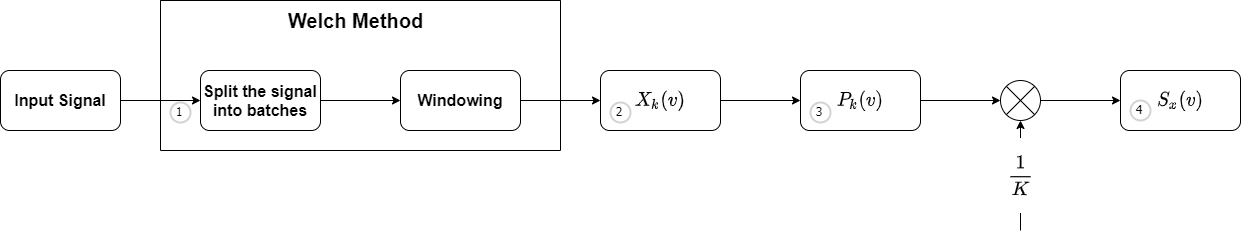
\includegraphics[width=400pt,keepaspectratio=true]{./fig/welchdiagram.png}
	% sekil3.eps: 0x0 pixel, 300dpi, 0.00x0.00 cm, bb=14 14 1155 740
	\caption{Flowchart of Power Spectral Density estimation via Welch's method \cite{jwo2021windowing}.}	
	\label{welchdiagram}
\end{figure}

By segmenting and window overlapping the data, the Welch method can increase the resolution and also reduce both the variance and bias of the spectral estimation \cite{stoica2005spectral,al2010advanced,zerdani2020inter}. The mechanism of adding window overlaps on the signal, which is similar to noise removal with the recursion algorithms, results a better Signal-to-Noise Ratio (SNR) in high noise data \cite{jwo2021windowing,jin2020intelligent,irvine2002introduction}. Welch's PSD estimation with Hamming window for fault diagnosis in induction motors outperforms FFT and periodogram methods in terms of robustness and accuracy due to reduced bias and variance \cite{ayhan2003case}.

\begin{figure}[!h]
	\centering
	\frame{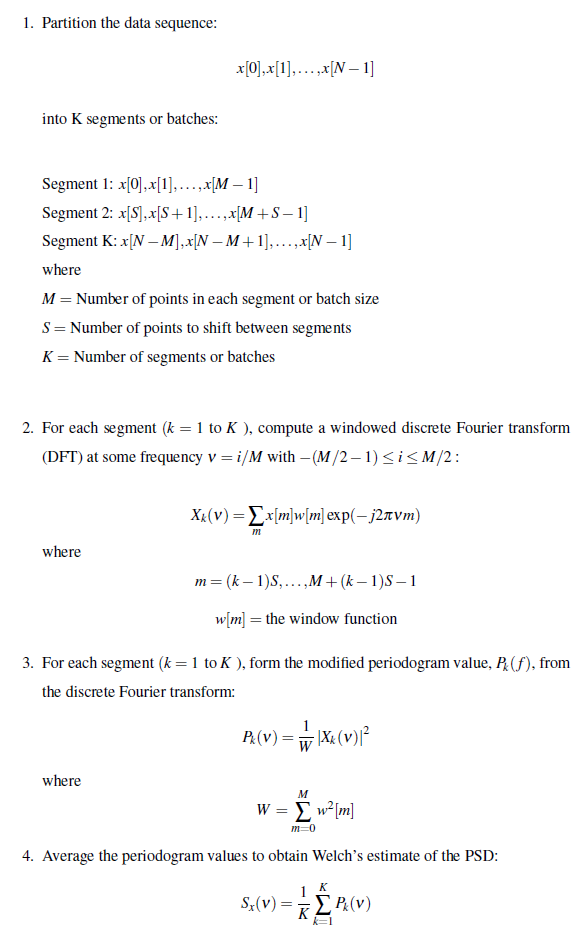
\includegraphics[width=400pt,keepaspectratio=true]{./fig/welch.png}}
	% sekil3.eps: 0x0 pixel, 300dpi, 0.00x0.00 cm, bb=14 14 1155 740
	\vspace{1cm}
	\caption{Algorithm of Power Spectral Density estimation via Welch's method \cite{solomon1991psd}.}	
	\label{welch}
\end{figure}
\pagebreak

\section{Data-driven fault diagnosis techniques}
Model and signal-based techniques have been applied successfully for many years in condition monitoring and fault diagnosis studies in induction motors. Although these approaches have their own advantages, they require a certain level of field expertise. With the establishment of the Industry 4.0 phenomenon, the increasing data size in industrial applications in recent years and the developments in the technologies of the hardware that will store and process this data form the infrastructure for data-oriented approaches. The fact that there has been vast academic interest in machine learning techniques, which are also defined as artificial intelligence, especially in the last ten years, causes an increase in industrial applications.

Increasing data-driven studies in the induction motors will be examined under classical machine learning and deep learning methods in this study. 

\subsection{Classical machine learning methods}

The state information of the motor contained in the current signal usually requires the processing of the signal. Fault diagnosis can be made with classical machine learning methods by processing the signal with statistical approaches in the time and frequency domains and approaches to extracting characteristics at certain frequencies in the frequency domain. 

Machine learning methods can be divided into supervised, unsupervised and semi-supervised according to training approaches. In supervised learning, the model is trained by giving the class information about the data to be processed as input, and the predicted class is given as a certain probability value as the model output. Within the scope of the thesis, supervised machine learning models were trained with a label indicating the motor status with the current signal.

\subsubsection{Naive Bayes}

Naive Bayes is a classification method based on the assumption that each feature is independent according to the class parameter \cite{friedman1997bayesian}. Outputs a probabilistic prediction of the target class for an unknown observation with its characteristics and class information input \cite{lowd2005naive}. Although it is simple in structure, it can be considered as a benchmark model in classification studies because it gives very fast and effective results even when the independence assumption is violated \cite{martin2018experimental}. 

\subsubsection{k-Nearest Neighbors}

One of the simplest machine learning methods, kNN can give very good results despite its simple structure and easy application. Even if the data set is large, the nearest neighbors can be found quickly and classification can be made \cite{shalev2014understanding}.

It works on the assumption that observations with similar attributes are more likely to produce similar results \cite{richman2011multivariate}. As a non-parametric method kNN performs classification based on the number or distance of the Nearest Neighbor in the data set.

\subsubsection{Support Vector Machines}

SVM as a supervised machine learning method is widely applied in regression problems and generally in classification problems. The main concept of SVM is locating a hyperplane that separates and classifies the datasets. The margin defines the support vectors of the datasets as it is the closest point to the hyperplane. Classification is accomplished by finding the hyperplane between the classes.

Besides performing linear classification, SVMs can efficiently perform nonlinear classification using various kernel functions. Kernel selection is quite important as it directly affects classification performance \cite{liu2018artificial}. There are many kernel and SVM architecture options for various problems in the literature. On the other hand, the performance of SVM algorithms is limited as the computational load increases with the increase in the number of samples \cite{haykin2010neural}. 

\subsubsection{Multi Layer Perceptron}

MLP is basically a learning structure consisting of input, output and hidden layers. The input layer is the layer where the input signals arrive and the output layer is the layer where the output signals depart. The layers other than input and output layers are called hidden layers. All layers in MLP are made up of neurons. These parts are called neurons because the structure of the brain's neurons to receive input and transmit an output by processing this input is imitated. In MLP, the output of each layer becomes the input of the next layer. The inputs to each neuron are multiplied by a weight and summed, and a weight (bias) is added to the value found. The value reached is passed through an activation function while being transmitted to the next layer. These processes are repeated from the input layer to the output layer. This process is the forward propagation part of MLP \cite{haykin2010neural}. Initially, the feed-forward stage takes place with randomly determined weights and an estimated output value is calculated for each signal. Each estimated output value calculated in this way contains errors. The weights are updated according to the errors to try to reduce the error. This process is performed starting from the output layer to the input layer. This part of the MLP is called backpropagation \cite{haykin2010neural}. During this update process, how much the weights will be updated is determined by the learning rate. The number of times these operations will be repeated for all data is expressed as the epoch. For how many data forward propagation and backpropagation will be applied together is represented by the batch size.

\subsubsection{Ensemble Learning}
Each model is developed based on certain assumptions and errors that occur as a result of these assumptions. It is aimed to minimize the total error by combining the predictions with a kind of voting method between training multiple models and their outputs \cite{alpaydin2020introduction,sewell2011ensemble}. The practice of employing multiple classification models and combining their predictions in this way is called ensemble learning.
\subsubsubsection{Random Forest}
Bagging, which is a voting method, can be defined as creating different variations by changing a dataset slightly and combining the outputs of each model after trained on a different variation \cite{alpaydin2020introduction,sewell2011ensemble}. As a refinement of bagged trees, Random Forest mainly aims to improve bagging by decorrelating the trees \cite{breiman2001random}. The procedure of voting for the most popular class after a large number of trees has been created is called random forests \cite{breiman2001random}.

\subsubsubsection{XGBoost}
The most common ensemble method, boosting provides sequential learning of the predictors and can be considered as a model averaging \cite{sewell2011ensemble}. As an iterative process, it continues to add classifier learner until a limit is reached by means of the number of models or accuracy \cite{alpaydin2020introduction}. XGBoost, a scalable machine learning algorithm for large-scale tree boosting, is a classifier variant with high performance in many different applications \cite{chen2021improved}.

\subsection{Deep learning methods}	

Deep learning, which is a sub-branch of machine learning, as its name implies, is artificial neural networks that deepen using many hidden layers. In classical machine learning, the artificial intelligence model requires feature engineering as a kind of preprocessing. Feature engineering requires specialized knowledge of statistical computing and signal processing, as well as knowledge of the general characteristics of the system. Deep learning methods, which provide a direct link between data collection and decision output by eliminating the manual feature extraction process, have attracted great attention in recent years.

As the importance of data spreading with Industry 4.0, manufacturers are starting to offer add-ons and services that will make it easier to access data for their products. For example, Wat Motor now offers special designs for vibration and temperature sensors that will be mounted into the motor, allowing monitoring of the status of its induction motors \cite{wat2021}. In the coming years, with the increase in the available data, deep learning methods will attract even more attention. While the performance of deep learning techniques increases in parallel to available data amount compared to classical machine learning methods, the trained model can be transferred to other applications with its transferability feature \cite{zhang2020deep}.

The increase in accessible data day by day, the interest of researchers from industry and academia that lead the development of new methods and approaches, and hardware developments such as Graphics Processing Unit (GPU), Tensor Processing Unit (TPU) and Field Programmable Gate Array (FPGA) that can process excessive calculations are the driving force of deep learning \cite{zhao2019deep,zhang2020deep}.

\subsubsection{1D-Convolutional Neural Networks}

CNN is a special case of feed-forward neural networks, with each hidden layer being a convolutional and pooling layer \cite{skowron2020convolutional}. Thanks to the convolutional layer, it provides a serious advantage in computational load \cite{skowron2020convolutional}. CNNs differ from Neural Networks in that they extract features of higher-order features from the input with convolutional processes \cite{chen2021improved}. The pooling layer is a layer that works in the direction of this idea by downsampling.

It is generally used in image processing and relies on the idea that an image does not need to be seen in its entirety to be perceived \cite{khan2018review}. Although it was originally a 2D structure, CNN structures of different dimensions were built afterwards and especially 1D structures employed in the analysis of time series signals such as current and vibration signals \cite{eren2019generic}.

\subsubsection{Long-Short Term Memory Networks}

Recurrent Neural Network (RNN) is a special type of neural network for sequential data. RNN also uses information from previous time steps, so it remembers the entire sequence \cite{sabir2019lstm}. In the backpropagation process for RNN, some problems may occur because the gradients are multiplied. These problems can be observed as the gradient becomes too small or too large \cite{sabir2019lstm}. To avoid these situations, LSTM, which has a memory cell and a special case of RNN, is used. Memory cell consists of forget, input and output gates. The forget gate determines how much previous step information should be remembered. The input gate expresses how much of the newly acquired information needs to be remembered. The output gate indicates how much memory will be used for the output of the relevant time step \cite{shenfield2020novel}.

\section{Performance evaluation}

Various metrics, which can be aggregated under binary or multi-class classification, are used to compare the performance of algorithms to be used in fault diagnosis \cite{canbek2017binary,seliya2009study}. In the diagnosis of asynchronous machine or their components, binary classification can be made as healthy or faulty condition, while multiple classification metrics should be used when separating two or more fault types.  Although there is no definite consensus for the metrics used in the comparison between the classification methods, the most frequently used metrics for multi-class classification will be examined in this section.

In order to create metrics, certain measures must be introduced. The confusion matrix shows the actual and predicted classification using certain measures. In the motor diagnostics specific, these four metrics can be defined as follows:
\begin{figure}[h]
	\centering
	\frame{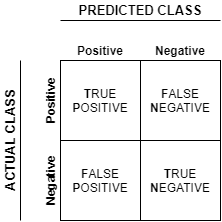
\includegraphics[width=100pt,keepaspectratio=true]{./fig/Confmat.png}}
	% sekil3.eps: 0x0 pixel, 300dpi, 0.00x0.00 cm, bb=14 14 1155 740
	\vspace{1cm}
	\caption{An example of Confusion Matrix.}	
	\label{confusion}
\end{figure}

True Positive (TP), the state where both the actual and predicted values are healthy,\\
False Positive (FP), the classification of the actually faulty condition as faulty, \\
False Negative (FN), the classification of the actually healthy motor as faulty,\\
True Negative (TN), the state where both the actual and predicted values are faulty.
\subsection{Precision \& Recall}

Precision refers to the ratio of samples that the classification method predicts as healthy to actually healthy samples, and shows how reliable the healthy motor prediction can be. Recall, on the other hand, expresses how many of the healthy motor samples were labelled correctly as a result of the classification and shows the model's ability to find the healthy motor. 
\begin{eqnarray}
\text{Precision} &=& \displaystyle\frac{TP}{TP+FP}\\
\text{Recall} &=& \displaystyle\frac{TP}{TP+FN} 
\label{precision}
\end{eqnarray}
\subsection{Accuracy}

Accuracy, one of the most common model performance metrics, is an indicator of how well it can distinguish between healthy and faulty motors in the entire data set \cite{grandini2020metrics}. In general, the number of healthy state data is naturally higher in diagnostic applications that result in an unbalanced data set \cite{han2021deep}. In such a case, evaluating only with the accuracy metric may lead to catastrophic situations. 
\begin{equation}
\text{Accuracy} = \displaystyle\frac{TP + TN}{TP + FP + FN + TN} 
\label{accuracy}	
\end{equation}
\subsection{F-measure}
As a metric based on Recall and Precision, F-Measure allows better inference than accuracy on classification performance, especially on unbalanced datasets \cite{he2009learning}. In multi-class classification case F-measure needs to be modified as Macro F-measure by averaging each and every class' F-measure.
\begin{eqnarray}
\text{F-measure} &=& 2\cdot\displaystyle\frac{Recall\cdot Precision}{Recall + Precision}\\
\text{Macro F-measure} &=& \displaystyle\frac{1}{C}\cdot \displaystyle\sum_{c_{i} \in C}\text{F-measure}({c_i})
\label{fmeas}	
\end{eqnarray}
where:\\
$c_{i} \quad$ is the reference class \\
$C \quad$ is the total number of classes\\
Especially in condition monitoring applications, fault alarms even though there is no fault increase the maintenance cost and at the same time, it can disrupt the operation. On the other hand, missing a fault condition can also damage equipment and disrupt the operation. The performance of the classification method is important in terms of optimizing both cases. F-measure can respond to this optimization as it contains components for these two states \cite{janssens2016convolutional,seliya2009study}.
\subsection{Cohen's Kappa}
Another metric that works well with unbalanced data, Cohen's Kappa correlates the estimated and actual values, taking into account the imbalance in the class distribution \cite{maaritwidmannalfredoroccato2021}. By removing the random dependency between the predicted and actual classification, enables to compare different classifiers \cite{grandini2020metrics}. 
\begin{equation}
\text{Cohen's Kappa} = \displaystyle\frac{c \cdot s-\displaystyle\sum_{k}^{C} p_{k} \cdot t_{k}}{s^{2}-\displaystyle\sum_{k}^{C} p_{k} \cdot t_{k}}
\label{kappa}	
\end{equation}
where:\\
$C\quad$ is the total number classes\\
$c=\displaystyle\sum_{k}^{K} C_{k k} \quad$ the total number of correctly predicted samples\\
$s=\displaystyle\sum_{i}^{K} \displaystyle\sum_{j}^{K} C_{i j}\quad$ the total number of samples\\
$p_{k}=\displaystyle\sum_{i}^{K} C_{k i}\quad$ the number of instances that class $k$ was predicted (column total)\\
$t_{k}=\displaystyle\sum_{i}^{K} C_{i k}\quad$ the number of instances that class $k$ actually presents (row total)

\subsection{Area Under the Curve}
Receiver operating characteristic (ROC) curve, which is another method widely used in binary classification performance measurement, shows the performance of classification methods in two dimensions \cite{fawcett2004roc}. To reduce this metric to one dimension, the area under the ROC curve (AUC) is calculated.

In multiclass classification problems, AUC values now transform into multiple binary classification values. The specified formula is used to reduce to a single numerical value \cite{fawcett2004roc}:
\begin{equation}
AUC_{total} = \displaystyle\sum_{c_{i} \in C} AUC(c_{i}) \cdot p(c_{i})
\label{auc}
\end{equation}
where:\\
$c_{i} \quad$ is the reference class \\
$C \quad$ is the total number of classes\\
$p(c_i) \quad$ is the prevalence of the reference class in the dataset\\
$AUC(c_{i}) \quad$ is the area under the class reference $ROC$ curve for $c_{i}$

According to this formula, AUC values are calculated by creating a ROC curve for each reference class, and the $AUC_{total}$ value is obtained by weighting it with the prevalence of the reference class \cite{fawcett2004roc,he2009learning}. The advantage of this method is that it is easily computable and is derived directly from reference class ROCs \cite{fawcett2004roc}.